\documentclass[11pt,openright,oneside,french]{book}

\usepackage{etex}

\usepackage[utf8]{inputenc}
\usepackage[T1]{fontenc}
\usepackage{babel}

\usepackage[margin=1.5cm]{geometry}

\usepackage[dvipsnames,table]{xcolor}
\usepackage{tikz,tkz-tab,tkz-fct,tkz-base,tkz-euclide}

\usepackage{mathtools}

\pagestyle{empty}

\usepackage{fancyvrb}
\usepackage{fvrb-ex}
\fvset{framerule=0.75pt,frame=leftline,gobble=4,rulecolor=\color{red},fontsize=\small,xrightmargin=0.5\linewidth,numbers=left}
% gobble=4 sert à dire que les espaces de 4 sont à ignorer. Cela correspond à la tabulation

\begin{document}
Voici un exemple avec son code \LaTeX{} à côté : \bigskip

\begin{SideBySideExample}
    Si $\Delta > 0$ alors les deux racines sont :
    \begin{align*}
        x_1 &= \frac{-b - \sqrt\Delta}{2a}\\
        \shortintertext{et}
        x_2 &= \frac{-b + \sqrt\Delta}{2a}.
    \end{align*}
\end{SideBySideExample}
\vspace{1cm}

Si les exemples sont trop grands, on peut faire avec cet autre environnement :\bigskip

\begin{CenterExample}
    \begin{center}
        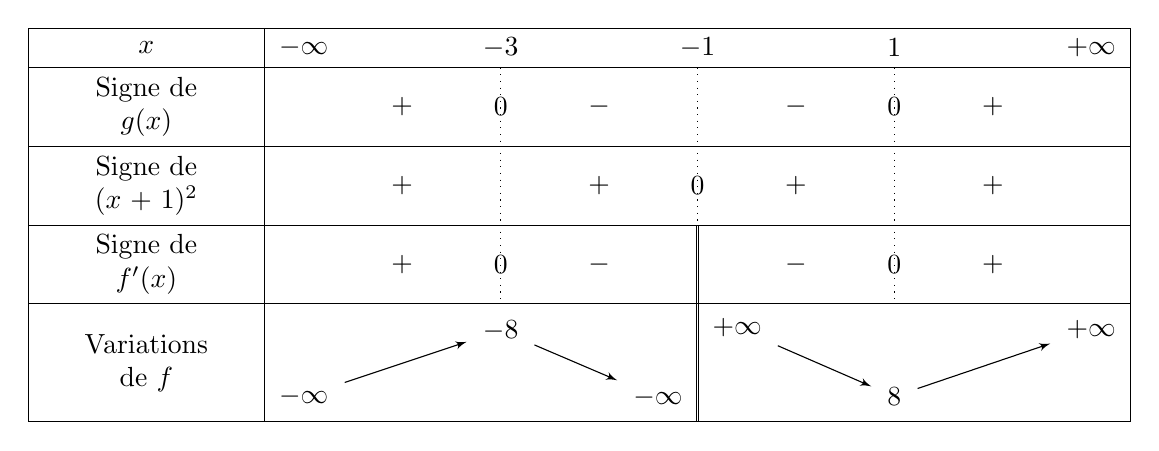
\begin{tikzpicture}
            \tkzTabInit[lgt=3,espcl=2.5]%
                {$x$/0.5,%
                Signe de \\ $g(x)$/1,%
                Signe de \\ $(x+1)^2$/1,%
                Signe de\\ $f'(x)$/1,%
                Variations\\ de $f$/1.5}%
                {$-\infty$,$-3$,$-1$,$1$,$+\infty$}
            \tkzTabLine{,+,z,-,t,-,z,+}
            \tkzTabLine{,+,t,+,z,+,t,+}
            \tkzTabLine{,+,z,-,d,-,z,+}
            \tkzTabVar{-/$-\infty$,+/$-8$,-D+/$-\infty$/$+\infty$,-/$8$,+/$+\infty$}
    	\end{tikzpicture}
    \end{center}
\end{CenterExample}


\end{document}
